\documentclass{article}

\usepackage{graphicx}
\usepackage[margin=2cm]{geometry}
\usepackage{verbatim}
\usepackage[export]{adjustbox}

\begin{document}

\newcommand{\modefont}[1]{\texttt{#1}}
\newcommand{\mnocheck}{\modefont{nocheck}}
\newcommand{\mnonstrict}{\modefont{nonstrict}}
\newcommand{\mstrict}{\modefont{strict}}

%% ---
\subsection*{Figure 3: Records per Hour}

Plot from \texttt{code/row-distribution.rkt}, which uses the dataset
\texttt{out/row-distribution.rktd}, which comes from running
\texttt{prepare.rkt --mode main}.

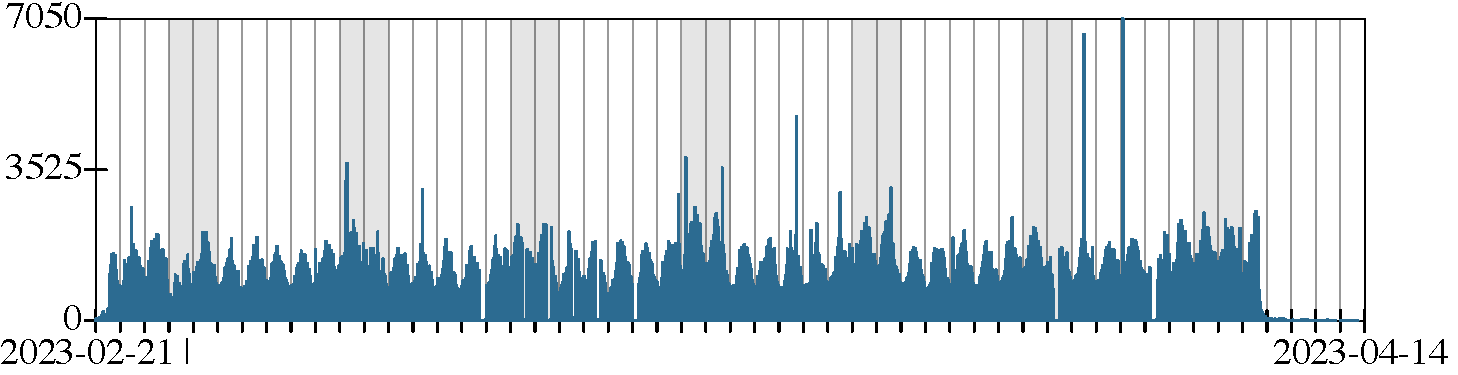
\includegraphics[width=\columnwidth]{out/row-distribution.pdf}

Lines 1-2 of \texttt{out/overview.txt} (output of \texttt{prepare.rkt --mode main})
give the reason for sending:

\begin{verbatim}
 1504736 total logs = 1341348 nocheck + 156883 nonstrict + 6505 strict
  508572 due to module switch
\end{verbatim}


%% ---
\subsection*{Table 2: Size of Analyzed Code}

From \texttt{out/summary-of-size-distributions.rktd},\\
which is the output of \texttt{code/sdupdate.rkt}\\
on \texttt{out/size-distributions.rktd}:

{\footnotesize
\verbatiminput{out/summary-of-size-distributions.rktd}
}

\begin{minipage}{0.5\columnwidth}
  \textbf{Lines:}\\
  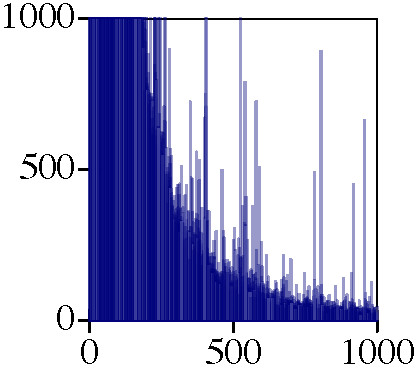
\includegraphics[width=\columnwidth]{out/lines-distribution.pdf}
\end{minipage}\begin{minipage}{0.5\columnwidth}
  \textbf{Edit Range:}\\
  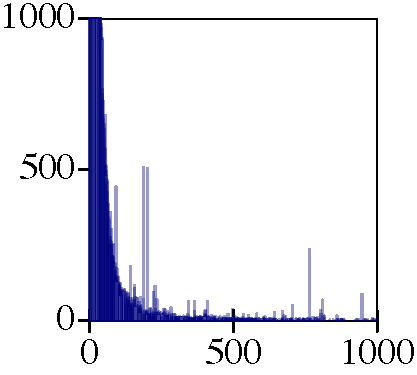
\includegraphics[width=\columnwidth]{out/editrange-distribution.pdf}
\end{minipage}


%% ---
\subsection*{Table 3: Session Size}

See previous section for mean, stddev, median, and P99.

\begin{minipage}{0.5\columnwidth}
  \textbf{Timespan:}\\
  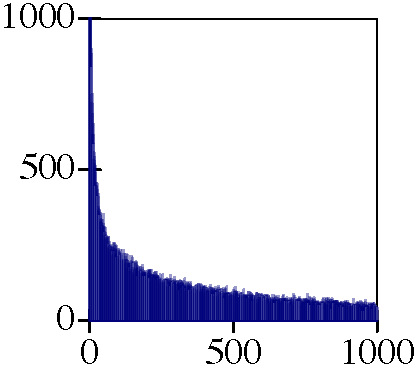
\includegraphics[width=0.4\columnwidth]{out/timespan-distribution.pdf}
\end{minipage}\begin{minipage}{0.5\columnwidth}
  \textbf{Event Count / Record Count:}\\
  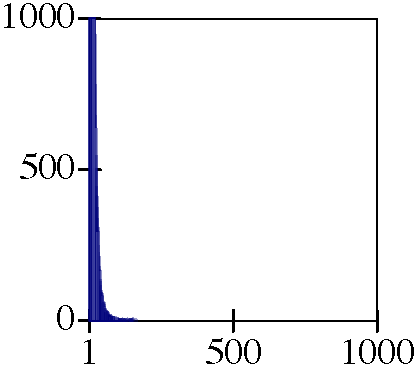
\includegraphics[width=0.4\columnwidth]{out/event-count-distribution.pdf}
\end{minipage}


%% ---
\subsection*{Table 4: Current Type Errors and Background Errors}

Lines 3-8 of \texttt{out/overview.txt}:

\begin{verbatim}
 72235735 total forced strict type errors, 37027281 in module,
 curr 1111178 in edit regions,
 olde 938500 in edit regions
 595137 total type errors, 289698 in module,
 curr 14917 non-stx + 16007 syntax in edit regions,
 olde 13836 non-stx + 28565 syntax in edit regions
\end{verbatim}


%% ---
\subsection*{Figure 4: Overview of Type Analysis Modes}

Line 1 of \texttt{out/overview.txt} partitions logs by mode:

\begin{verbatim}
 1504736 total logs = 1341348 nocheck + 156883 nonstrict + 6505 strict
\end{verbatim}

Lines 9-13 of \texttt{out/overview.txt} partition sessions and report on upgrades and downgrades,
\emph{but} the final two numbers are incorrect (upgrade and downgrade) because they include
module switches:

\begin{verbatim}
 347598 sessions
  346956 single mode = 313509 nocheck + 32902 nonstrict + 545 strict
  512 multi mode projects
  341 mode upgrades
  320 mode downgrades
\end{verbatim}

Correct up/down-grade numbers are in \texttt{out/downgrade-count.txt},
which is the output of \texttt{code/downgrade-count.rkt} after running
the following commands to generate data:

\begin{verbatim}
PLTSTDERR="error info@luau" racket prepare.rkt --mode divide-sessions
PLTSTDERR="error info@luau" racket prepare.rkt --mode session-query
PLTSTDERR="error info@luau" racket prepare.rkt --mode aggregate-te
\end{verbatim}

% \includeverbatim{out/downgrade-count.txt}

% TODO


%% ---
\subsection*{Figure 5: Type and Background Errors Grouped by Mode}

These plots come from \texttt{code/error-by-mode.rkt}, which uses
hard-coded data from \texttt{out/overview.txt}:

{ \newcommand{\labelbars}[1]{\begin{tabular}[t]{l@{}l} \raisebox{2ex}{\begin{tabular}[t]{r}\mnocheck{}\\\mnonstrict{}\\\mstrict{}\end{tabular}} & #1 \end{tabular}}
  \begin{tabular}[t]{cc}
    Type errors & Background errors \\
    \labelbars{\includegraphics[width=0.20\columnwidth,valign=M]{out/error-by-mode-te.pdf}}
    & \labelbars{\includegraphics[width=0.20\columnwidth,valign=M]{out/error-by-mode-fs.pdf}}
  \end{tabular}
}


%% ---
\subsection*{Table 5: Specific Errors in Edit Range}

Output from \texttt{code/type-error-survival.rkt}
run on \texttt{code/type-error-survival-ss-*.rktd}:

TODO


%% ---
\subsection*{Table 6: Type Error Popularity}

Output from \texttt{code/type-error-count.rkt}
run on \texttt{code/te-editrange-ss-*.rktd}:

TODO


\subsubsection*{Internal Limits, Code Too Complex}

Data from \texttt{out/ctc-info.txt}, which comes from
\texttt{prepare.rkt --mode main}:

{\footnotesize
\verbatiminput{out/ctc-info.txt}
}


%% ---
\subsection*{Figure 6: Type Error Density}

Plot output from \texttt{code/error-count.rkt}
on \texttt{out/error-density-ss-*.rktd}.
(It also prints text output.):

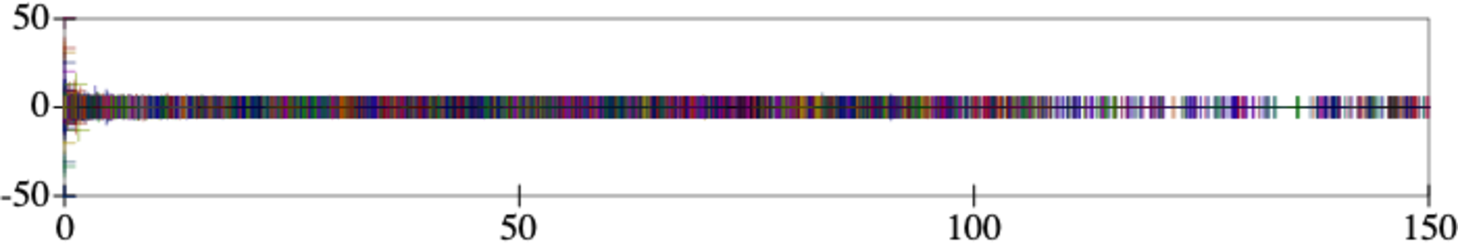
\includegraphics[width=0.8\columnwidth]{out/error-count-nocheck-row--te-density-diff.pdf}
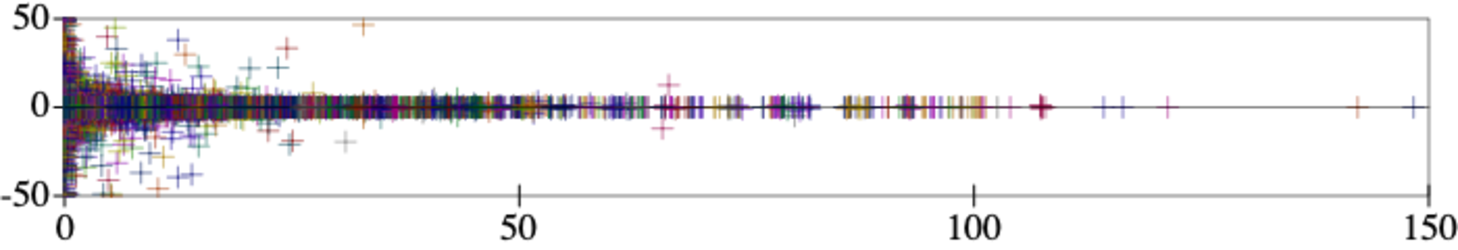
\includegraphics[width=0.8\columnwidth]{out/error-count-nonstrict-row--te-density-diff.pdf}
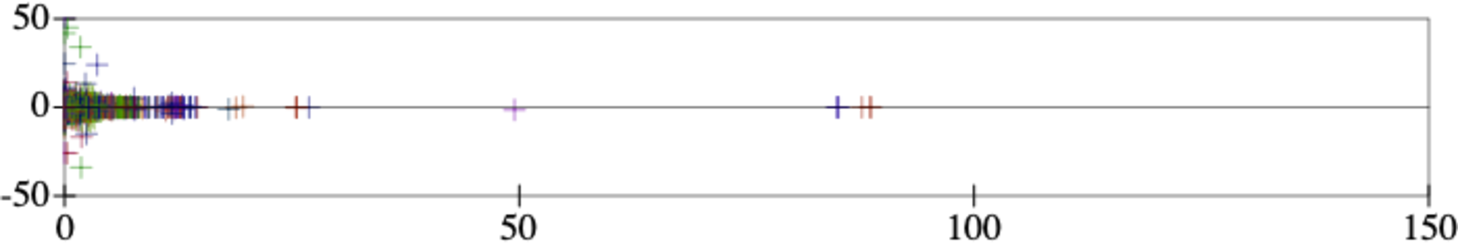
\includegraphics[width=0.8\columnwidth]{out/error-count-strict-row--te-density-diff.pdf}


\subsection*{Figure 7: Type Error Density}

Shuffled text output from \texttt{code/error-count.rkt}
on \texttt{out/error-density-ss-*.rktd}:

\begin{verbatim}
TE
  nocheck & 48378 & (\pct{46.83}) & 9440 & [\pct{9.14}] & 45479 & [\pct{44.03}] \\
FS
  nocheck & 270763 & (\pct{36.99}) & 238696 & [\pct{32.61}] & 222588 & [\pct{30.41}] \\
TE mod
  nocheck & 20085 & (\pct{49.83}) & 906 & [\pct{2.25}] & 19317 & [\pct{47.92}] \\
FS mod
  nocheck & 259865 & (\pct{39.09}) & 175643 & [\pct{26.42}] & 229271 & [\pct{34.49}] \\
TE
  nonstrict & 19491 & (\pct{39.63}) & 9567 & [\pct{19.45}] & 20121 & [\pct{40.91}] \\
FS
  nonstrict & 35330 & (\pct{37.28}) & 29483 & [\pct{31.11}] & 29955 & [\pct{31.61}] \\
TE mod
  nonstrict & 13030 & (\pct{40.22}) & 5513 & [\pct{17.02}] & 13852 & [\pct{42.76}] \\
FS mod
  nonstrict & 33988 & (\pct{39.74}) & 20738 & [\pct{24.25}] & 30798 & [\pct{36.01}] \\
TE
  strict & 733 & (\pct{39.18}) & 368 & [\pct{19.67}] & 770 & [\pct{41.15}] \\
FS
  strict & 574 & (\pct{33.71}) & 561 & [\pct{32.94}] & 568 & [\pct{33.35}] \\
TE mod
  strict & 419 & (\pct{39.31}) & 230 & [\pct{21.58}] & 417 & [\pct{39.12}] \\
FS mod
  strict & 488 & (\pct{36.53}) & 344 & [\pct{25.75}] & 504 & [\pct{37.72}] \\
\end{verbatim}



\end{document}
